\documentclass[aspectratio=169]{beamer}
\usepackage[utf8]{inputenc}
\usepackage[T1]{fontenc}
\usepackage{lmodern}
\usepackage{listings}
\usepackage{xcolor}
\usepackage{graphicx}
\usepackage{booktabs}
\usepackage{verbatim}

% Theme and color scheme
\usetheme{Madrid}
\usecolortheme{default}

% Code highlighting
\lstset{
    language=C++,
    basicstyle=\ttfamily\small,
    keywordstyle=\color{blue}\bfseries,
    commentstyle=\color{green!60!black},
    stringstyle=\color{red},
    numberstyle=\tiny\color{gray},
    numbers=left,
    breaklines=true,
    showstringspaces=false,
    frame=single,
    backgroundcolor=\color{gray!10}
}

% JSON highlighting
\lstdefinelanguage{json}{
    basicstyle=\ttfamily\small,
    commentstyle=\color{green!60!black},
    stringstyle=\color{red},
    numberstyle=\tiny\color{gray},
    numbers=left,
    breaklines=true,
    showstringspaces=false,
    frame=single,
    backgroundcolor=\color{gray!10},
    string=[s]{"}{"},
    comment=[l]{//},
    morecomment=[s]{/*}{*/},
    literate=
        *{0}{{{\color{blue}0}}}{1}
        {1}{{{\color{blue}1}}}{1}
        {2}{{{\color{blue}2}}}{1}
        {3}{{{\color{blue}3}}}{1}
        {4}{{{\color{blue}4}}}{1}
        {5}{{{\color{blue}5}}}{1}
        {6}{{{\color{blue}6}}}{1}
        {7}{{{\color{blue}7}}}{1}
        {8}{{{\color{blue}8}}}{1}
        {9}{{{\color{blue}9}}}{1}
        {:}{{{\color{black}{:}}}}{1}
        {,}{{{\color{black}{,}}}}{1}
        {\{}{{{\color{black}{\{}}}}{1}
        {\}}{{{\color{black}{\}}}}}{1}
        {[}{{{\color{black}{[}}}}{1}
        {]}{{{\color{black}{]}}}}{1},
}

% CMake highlighting
\lstdefinelanguage{cmake}{
    basicstyle=\ttfamily\small,
    commentstyle=\color{green!60!black},
    stringstyle=\color{red},
    numberstyle=\tiny\color{gray},
    numbers=left,
    breaklines=true,
    showstringspaces=false,
    frame=single,
    backgroundcolor=\color{gray!10},
    keywords={cmake_minimum_required, project, find_package, add_executable, target_link_libraries, set, if, endif, foreach, endforeach, function, endfunction, macro, endmacro, include, add_subdirectory, target_include_directories, target_compile_definitions, option, configure_file, install, FetchContent_Declare, FetchContent_MakeAvailable, FetchContent_GetProperties},
    keywordstyle=\color{blue}\bfseries,
    comment=[l]{\#},
    string=[b]",
    morestring=[b]',
    sensitive=false,
}

% Title page information
\title{Introduction to Intrusive \& Visual Profiling}
\subtitle{Focusing on Constrained Environments}
\author{Lukáš Růžička}
\institute{Prague C++ Meetup}
\date{2025 07 29}



\begin{document}



% Title slide
\frame{\titlepage}

\begin{frame}{Table of Contents}
\tableofcontents[hideallsubsections]
\end{frame}

% Current section
\AtBeginSection[ ]
{
\begin{frame}{Outline}
    \tableofcontents[currentsection]
\end{frame}
}



\section{Personal introduction}

\begin{frame}
    Hi, I'm Lukas.

    Please feel free to ask questions immediately, or save them for the end (ideally remember the context using the page number in the corner).

    I like the concept of these meetups and wanted to contribute beside just consuming others' presentations. But what to share and how?

    About 7 years ago, I solved one of my first programming tasks using the `nvtx` library and a Visual Studio addon that received and displayed the profiling data.

    The issue was: one thread was pushing to a queue while another was popping from it. When the queue was empty, there was a "timed wait" (probably using `std::condition\_variable` or similar). This was called inefficiently - it never terminated except by timeout, which I observed through visualising the profiling results.

    Personally I find profiling enjoyable, and I hope you will enjoy this talk.

\end{frame}



\section{Structure of the talk}

\begin{frame}
    My planned approach\footnote{confirmed in this discord thread with this poll https://discord.com/channels/1077146284143673354/1387733811818922014/1387736431883063346}:

    \begin{itemize}
        \item First, I'll describe my experience with "external" libraries/frameworks/tools:
        \begin{itemize}
            \item nvtx
            \item Tracy
            \item perf + flamegraphs
            \item Mention some others I've heard off but never used (Intel VTune Profiler, Clang XRay, ...)
        \end{itemize}
        \item Then explain what didn't work for me and what I needed differently
        \item This led me to start writing my own library for this purpose (second half of the presentation: cxxet)
    \end{itemize}

\end{frame}



\section{How to understand mentioned terms}

\begin{frame}{Application profiling}
    To profile an application means to somehow measure its performance, resource usage, etc. in order to identify bottlenecks, potential optimization opportunities, and so on.

    Some related quotes:
    \begin{itemize}
        \item "Premature optimization is root of all evil."
        \item "You don't improve what you don't measure."
    \end{itemize}

\end{frame}
\begin{frame}{Non-intrusive profiling}
    Measuring performance without requiring any source code modification of the target application. This is usually done by attaching a tool to a running application, which then collects data about its performance, resource usage, and so on.

    Examples:

    \begin{itemize}
        \item `time ...' - the simplest and crudest option (for unix OSes)
        \item `perf' (in tandem with `Flame Graph' tools for the "visual" part)
        \item Microsoft Visual Studio Profiler (e.g. https://learn.microsoft.com/en-us/visualstudio/profiling)
    \end{itemize}

\end{frame}

\begin{frame}{Intrusive profiling}
    Measuring performance by modifying the application's source code - typically by incrementally adding markers/logging/etc. based on results from previous iterations.

    This is very similar to "printf debugging", which can also serve as the simplest form of this type of profiling - printing measured times to standard output, logs, and similar.

\end{frame}

\begin{frame}{Visual profiling}
    Displaying results using some UI, for example `chrome://tracing` or `perfetto.ui`.

    The opposite might be "basic" (e.g. textual) display of collected data such as `perf report`, or simple logging of time spent in some part of the code.

\end{frame}

\begin{frame}{Constrained environments}
    I apologize for the somewhat misleading name - specifically for the word "constrained" - generally in software development it is understood in connection with embedded systems, but that wasn't my case - my environment was indeed a "large" server, but the limitations (... constraints ...) were different - absence of `root' access (for perf) and internal architecture of the application.

    I would be happy if someone experienced in the `embedded' field would tell me what the typical limitations in this field are.

\end{frame}



\section{Established tools and frameworks}


\subsection{Nvtx}

\begin{frame}[fragile]{Nvtx usage example}{example code `examples/nvtx/main.cxx'}
    
    \begin{lstlisting}[language=C++]
#include <thread>
#include <nvtx3/nvtx3.hpp>

void some_function() {
  NVTX3_FUNC_RANGE(); // equivalent to e.g. `nvtx3::scoped_range fn{__FUNCTION__};'
  for (int i = 0; i < 6; ++i) {
    nvtx3::scoped_range loop{"loop iteration range"};
    // Make each iteration last for one ms:
    std::this_thread::sleep_for(std::chrono::milliseconds{1});
  }
}

int main(int, char **) {
  some_function();
}
    \end{lstlisting}

\end{frame}

\begin{frame}{Nvtx usage example}
    Windows host, linux target:

    \begin{enumerate}
        \item download and install it on windows host: https://developer.nvidia.com/nsight-systems/get-started\#Winx86
        \item download it for linux target (e.g. Ubuntu): https://developer.nvidia.com/nsight-systems/get-started\#Linuxx86
        \item install it: `sudo dpkg --install NsightSystems-linux-cli-public-2025.3.1.90-3582212.deb'
        \item compile the example: `\$ cd examples/nvtx \&\& ./build.bash'
        \item run it: `\$ time nsys profile build/nvtx\_example'
        \item add/remove markers in source code as needed
        \item go to step no. 4, etc.
    \end{enumerate}

\end{frame}

\begin{frame}{Nvtx usage example}{example output}
    \begin{figure}[h]
        \centering
        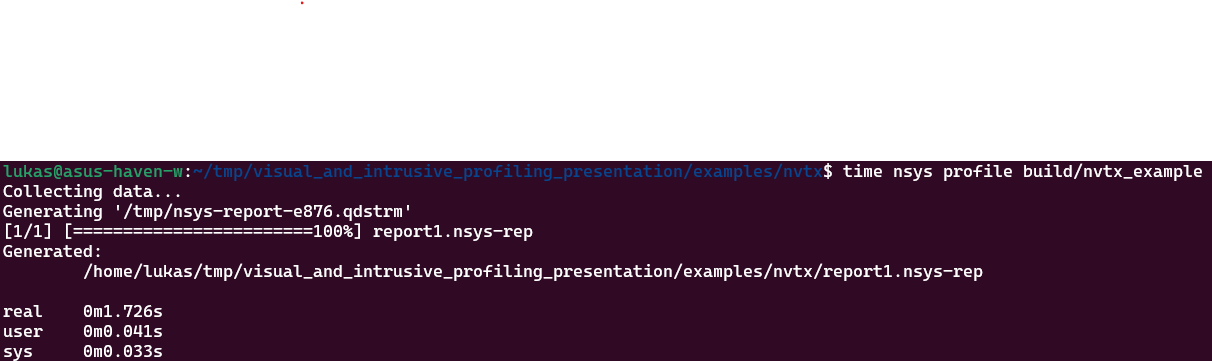
\includegraphics[width=\textwidth,height=0.7\textheight,keepaspectratio]{pics/nvtx/nsys_example.png}
        \caption{Application profiling via nsys and nvtx}
    \end{figure}

\end{frame}

\begin{frame}{Nvtx usage example}{displayed data}

    \begin{figure}[h]
        \centering
        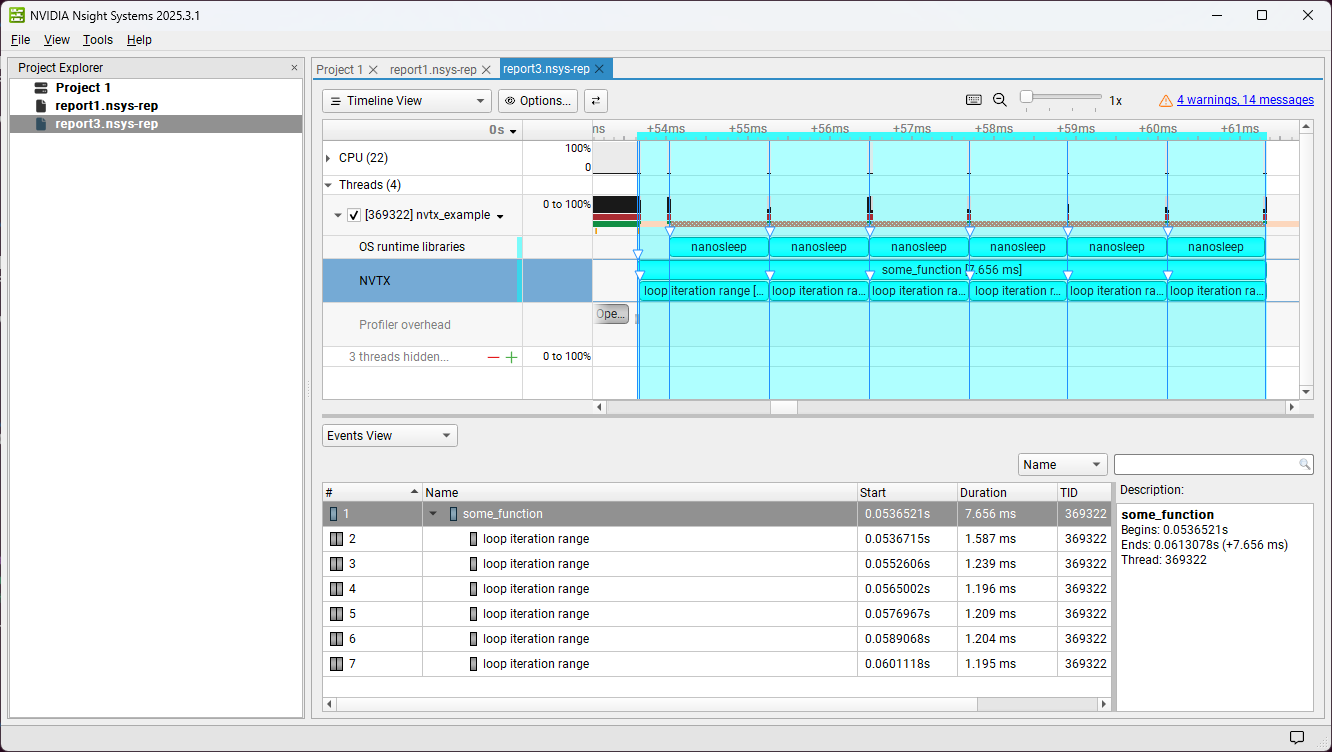
\includegraphics[width=\textwidth,height=0.7\textheight,keepaspectratio]{pics/nvtx/gui.png}
        \caption{Nsight Systems profiling gui}
    \end{figure}

\end{frame}

\begin{frame}{NVIDIA Nsight Systems + nvtx}
    Advantages:

    \begin{itemize}
        \item extensive framework, capable of much more than what I'm describing here
        \item ability to observe behavior in real time (when launched through the GUI - another "driver")
    \end{itemize}

    Disadvantages:

    \begin{itemize}
        \item the profiler (`nsys' in the example above) is a standalone application, which if not suitable/available, requires using another "driver" or providing your own one (see https://github.com/NVIDIA/NVTX/tree/release-v3/tools/sample-injection)
    \end{itemize}

    Further references:

    \begin{itemize}
         \item https://developer.nvidia.com/nsight-systems
         \item https://docs.nvidia.com/nsight-systems/UserGuide/index.html\#nvtx-trace
         \item https://github.com/NVIDIA/NVTX
    \end{itemize}

\end{frame}


\subsection{Tracy}

\begin{frame}[fragile]{Tracy usage example}{example code `examples/tracy/main.cxx'}
    
    \begin{lstlisting}[language=C++]
#include <thread>
#include <tracy/Tracy.hpp>

void some_function() {
  ZoneScoped; // equivalent to the `NVTX3_FUNC_RANGE();`
  for (int i = 0; i < 6; ++i) {
    ZoneScopedN("loop iteration range"); // equivalent to the
                                         // `nvtx3::scoped_range loop{...};`
    std::this_thread::sleep_for(std::chrono::milliseconds{1});
  }
}

int main(int, char **) { some_function(); }
    \end{lstlisting}

\end{frame}

\begin{frame}{Tracy usage example}
    All on linux (wsl2 Ubuntu):

    \begin{enumerate}
        \item build its gui (see section 2.3 in its documentation):
        \begin{itemize}
            \item `\$ cmake -B profiler/build -S profiler -DCMAKE\_BUILD\_TYPE=Release -DLEGACY=ON'
            \item `\$ cmake --build profiler/build --config Release --parallel'
        \end{itemize}
        \item compile the example: `\$ cd examples/tracy \&\& ./build.bash'
        \item run it: `\$ TRACY\_NO\_EXIT=1 build/tracy\_example'
        \item drain the collected data via gui `\$ profiler/build/tracy-profiler' and explore it
        \item adjust markers in the source code as needed
        \item repeat if needed: go to step no. 3
    \end{enumerate}

\end{frame}

\begin{frame}{Tracy usage example}{fresh gui}
    \begin{figure}[h]
        \centering
        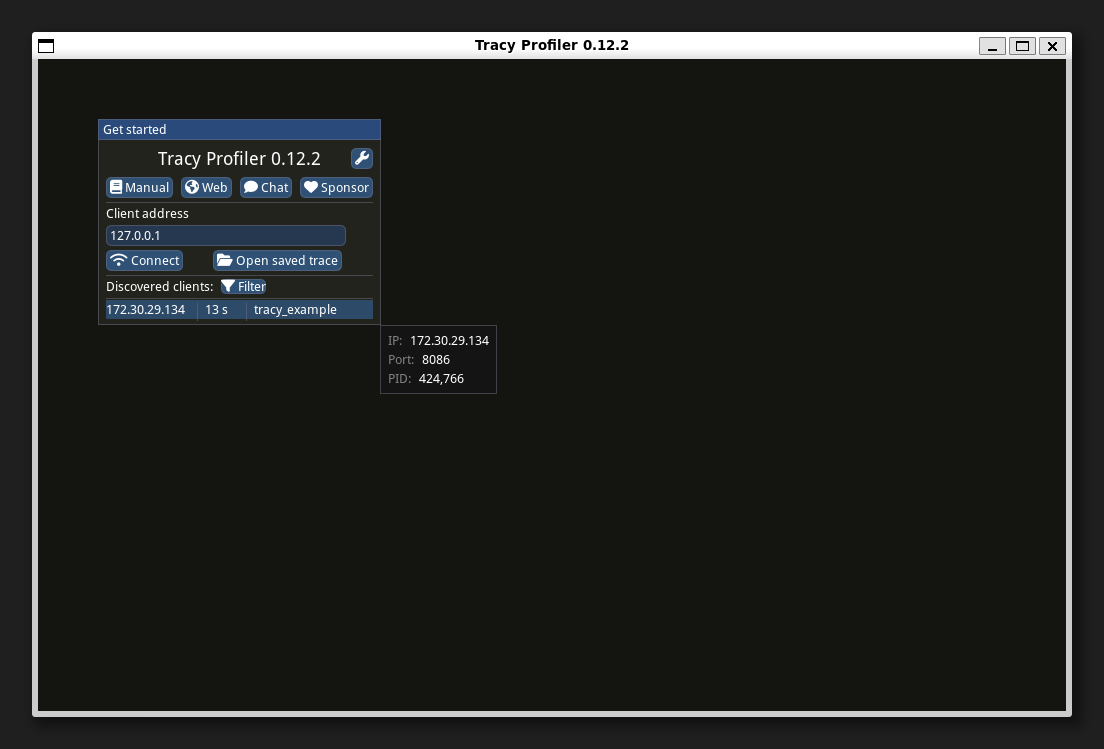
\includegraphics[width=\textwidth,height=0.7\textheight,keepaspectratio]{pics/tracy/gui1.png}
        \caption{Choosing process}
    \end{figure}

\end{frame}

\begin{frame}{Tracy usage example}{displayed data}

    \begin{figure}[h]
        \centering
        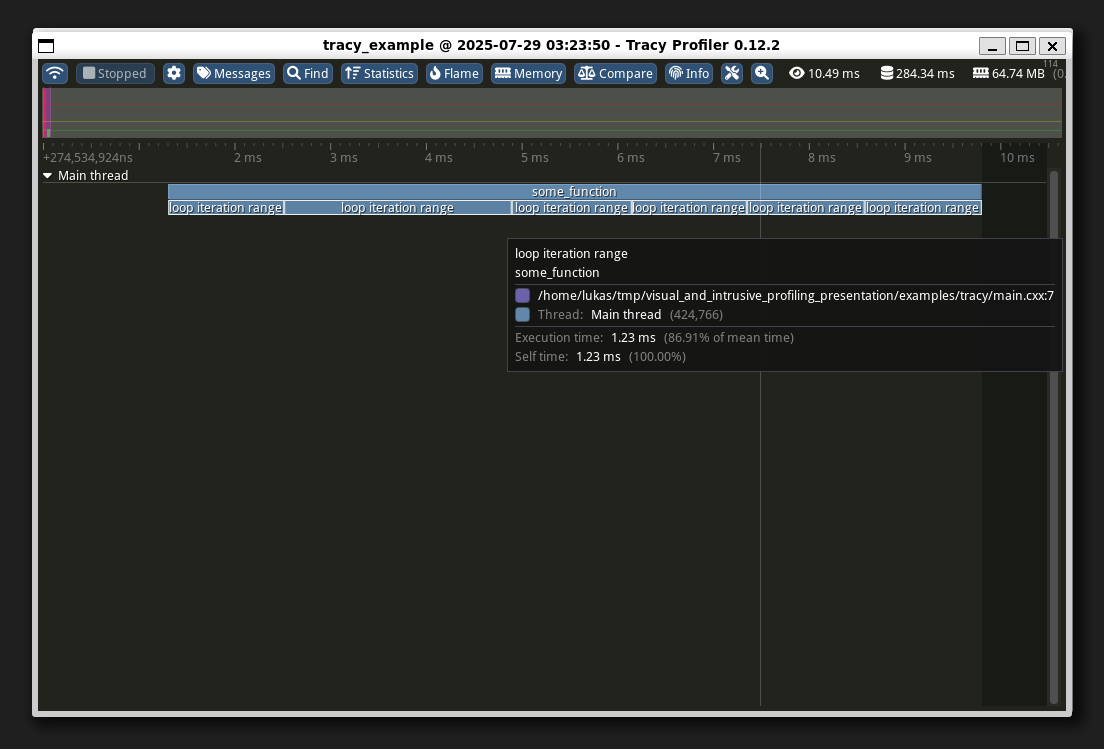
\includegraphics[width=\textwidth,height=0.7\textheight,keepaspectratio]{pics/tracy/gui2.png}
        \caption{Tracy gui}
    \end{figure}

\end{frame}

\begin{frame}{Tracy}
    Advantages:

    \begin{itemize}
        \item again, extensive framework, capable of far more than what I'm describing here
        \item no "profiling" application needed - on the profiled program side, it's sufficient to link the appropriate library (`libTracyClient.a'/`TracyClient' in the example above)
        \item ability to observe behavior in real time (in the gui)
    \end{itemize}

    Disadvantages:

    \begin{itemize}
        \item inability to export data to other formats
        \item focused on desktop/gui applications
        \item `TracyClient' library is robust but not very modifiable
    \end{itemize}

    Further references:

    \begin{itemize}
        \item https://github.com/wolfpld/tracy
        \item https://github.com/wolfpld/tracy/releases/latest/download/tracy.pdf
    \end{itemize}

\end{frame}


\subsection{Perf + FlameGraph}

\begin{frame}{Perf + FlameGraph}
    Just a quick mention: `perf'\footnote{https://perfwiki.github.io/main} is advanced sampling profiler for linux, and `Flame Graph' tools can be used to visualize collected results\footnote{https://github.com/brendangregg/FlameGraph?tab=readme-ov-file\#linux-perf\_events-1}.

\end{frame}


\subsection{Furher tools ...}

\begin{frame}
    There are more tools, which I don't have any experience with, and therefore I won't talk about them. Using some search engine would probably yield few more results, and among the top ones would be probably e.g.:

    \begin{itemize}
        \item Intel VTune Profiler\footnote{https://www.intel.com/content/www/us/en/developer/tools/oneapi/vtune-profiler.html}
        \item Clang XRay\footnote{https://llvm.org/docs/XRay.html}
        \item ...
    \end{itemize}

\end{frame}



\section{My (previous) situation}

\begin{frame}{My (previous) environment}
    Returning to the misleading "constrained environments" from the introduction: in my previous company, I needed/wanted to profile a web server application with roughly this architecture:

    \begin{enumerate}
        \item after startup, `fork()' was called and the parent terminated, the child continued by calling `setsid()'\footnote{process daemonization, equivalent to http://man7.org/linux/man-pages/man3/daemon.3.html}
        \item application initialization (reading configuration files, etc.)
        \item opening socket for receiving requests
        \item loop for accepting incoming requests, which were passed for processing to a `fork'ed child process (which terminated after sending the response)
    \end{enumerate}

    The environment was initially very inflexible - old `Debian' on a "shared" machine:
    
    \begin{itemize}
        \item shared development environment for all developers
        \item no possibility to install or directly use tools (such as `perf')
    \end{itemize}

\end{frame}

\begin{frame}{Working around that}
    Using `perf' or `nvtx' wasn't feasible, and `Tracy' out of the box was unusable too - those `forks' (see previous slide) caused both processes to send their data via the `TracyClient' connection to the "collector" and it simply crashed.

    I managed to "bend" `TracyClient' by using a few compilation switches - namely `TRACY\_DELAYED\_INIT' and `TRACY\_MANUAL\_LIFETIME' \footnote{see section 2.1.8 in its documentation https://github.com/wolfpld/tracy/releases/latest/download/tracy.pdf} - `TracyClient' was then initialized only in the "second" `fork()'ed child (4th point in the previous slide), where it juggled with the `TRACY\_PORT' value - it had to use different port numbers for each `fork'ed child.

    However, it had at least one practical drawback: no code used both before and after this delayed initialization could contain any markers, etc. because in the "first" phase they would cause a crash (most probably due to accessing uninitialized data in `TracyClient' implementation). Examples of such features included logging functions, DB accessing functions, etc.

\end{frame}

\begin{frame}{My (previous) environment v2.0}
    Eventually, the application got "containerized" and the `daemonization' (point 1 in the prev. slide) became unnecessary, but the second `fork()' (per each incoming request; point 4 over there) was left unchanged.

    IMHO, "healthier" solutions would be either:

    \begin{itemize}
        \item not to `fork()', but simply introduce a thread pool,
        \item factor out the loop with new connection/request accepting to a separate application, which would still `fork()', but would call `execv("my\_web\_server", ...)' for each separate request, effectively making the `my\_web\_server' utility-like.
    \end{itemize}

    Unfortunately, doing either of those wasn't feasible at the time, so the `TracyClient' setup was left unchanged because of that.

\end{frame}

\begin{frame}{Minimalalistic tracing library}
    In the end, the "adjusted" `TracyClient' partially and sufficiently fulfilled my needs, but the overall experience was bad. Hence the idea for writing my own library for that purpose arose - which eventually led me to start writing the `cxxet' library https://github.com/Ruzovej/cxxet (abbreviation of "C++ easy tracing").
    
    Maybe it's little ironical that before doing so, I stopped working at this company.

\end{frame}


% TODO continue checking this here ...
\section{C++ easy tracing}

\begin{frame}{cxxet}{Requirements}
    The goal of this library is to:
    
    \begin{itemize}
        \item \label{easy_usage} provide an easy way how to intrusively mark up source code to generate profiling data,
        \item \label{writing_out_data} hand over the collected data as simply as possible,
        \item \label{fork_handling} be able to handle `fork()'s (and similar stuff) without any tweaking\footnote{as opposed to `Tracy'},
        \item \label{no_external_wrapper} not require any external application wrapper\footnote{as opposed to `nvtx'}.
    \end{itemize}

    Compared to the other frameworks (e.g. `NVIDIA Nsight Systems', `Tracy'), it doesn't have any "visualizing" capabilities, and this added one last requirement:

    \begin{itemize}
        \item \label{data_format} output the collected data using some "standard" format.
    \end{itemize}

\end{frame}

\begin{frame}{cxxet}{Missing features}
    Compared to the competition, it lacks at least:

    \begin{itemize}
        \item ability to observe the generated traces in real time (not planning to implement this),
        \item maturity (it's still new, and I didn't have as much time as I wanted to work on it),
        \item few critical features needed for smooth adoption by anyone else:
        \begin{itemize}
            \item documentation,
            \item ability to run on other platforms other than x86-64 Linux\footnote{maybe it would work on aarch Linux too, but right now definitely not on Windows}.
        \end{itemize}
    \end{itemize}

    In other words, "help wanted"! I would be glad for any feedback\footnote{partially fulfilled by this talk?}, not even dreaming about code contribution from others.

\end{frame}


\subsection{Features}

\begin{frame}{cxxet features}{Ease of usage?}
    Regarding the \hyperlink{easy_usage}{ease of usage requirement}, there are at least two factors:

    \begin{itemize}
        \item obtaining the library,
        \item marking up the source code.
    \end{itemize}

\end{frame}

\begin{frame}[fragile]{cxxet features}{Obtaining the library}
    Currently, the easist way is to use `cmake' and its `FetchContent' module:

    \begin{lstlisting}[language=cmake]
...
FetchContent_Declare(
    cxxet
    GIT_REPOSITORY  git@github.com:Ruzovej/cxxet.git
    GIT_TAG         some_value # branch/tag name, e.g. `main'
)
FetchContent_MakeAvailable(cxxet)

add_executable(your_target ...)
target_link_libraries(your_target PRIVATE cxxet::trace)
...
    \end{lstlisting}

    For more inspiration, see two related examples within the library repository: https://github.com/Ruzovej/cxxet/tree/main/examples/cmake\_fetch\_content

\end{frame}

\begin{frame}{cxxet features}{Marking up the source code}
    All the basic functionality is in the file `cxxet/all.hxx'\footnote{https://github.com/Ruzovej/cxxet/blob/main/include/all/cxxet/all.hxx}.

    In general, the source code repository contains many examples\footnote{https://github.com/Ruzovej/cxxet/tree/main/examples}. Those demonstrate how to use all provided features, including (not yet introduced, but \hyperlink{fork_handling}{above mentioned}) "sink diversion"\footnote{https://github.com/Ruzovej/cxxet/tree/main/examples/usage/sink\_diversion}.

\end{frame}

\begin{frame}[fragile]{cxxet features}{Marking up the source code - comparison}
    When compared to e.g. `nvtx', helper classes and macros which provide the desired markup functionality are very similar, e.g.:

    \begin{lstlisting}[language=C++]
#include <cxxet/all.hxx> // formerly `#include <nvtx3/nvtx3.hpp>'
void some_function() {
  CXXET_mark_complete(__FUNCTION__); // formerly `NVTX3_FUNC_RANGE();'
  for (int i = 0; i < 6; ++i) {
    CXXET_mark_complete("loop iteration range"); // formerly `nvtx3::scoped_range loop{"loop iteration range"};'
...
    \end{lstlisting}

    And similar applies for `Tracy'.

\end{frame}

\begin{frame}[fragile]{cxxet features}{Marking up the source code - best practice(s)}
    It's recommended to pay the cost for `thread\_local' buffer allocation before submiting any marker:

    \begin{lstlisting}[language=C++]
#include <cxxet/all.hxx>
int main(int argc, char const **argv) {
  CXXET_sink_thread_reserve(); // <--
  // ...
  std::thread t{[]() {
    CXXET_sink_thread_reserve(); // <--
    // ...
    CXXET_sink_thread_flush(); // not necessary - happens implicitly in the internal `thread_local' object destructor
  }};
  // ...
  t.join();
}
    \end{lstlisting}

\end{frame}

\begin{frame}[fragile]{cxxet features}{One visual example - code}
    Simplified snippet from `examples/usage/complete/1.cxx'\footnote{https://github.com/Ruzovej/cxxet/blob/main/examples/usage/complete/1.cxx} follows:

    \begin{lstlisting}[language=C++]
#include "cxxet/all.hxx"

static void pyramid(int const level) {
  CXXET_mark_complete(__FUNCTION__);
  std::this_thread::sleep_for(std::chrono::milliseconds(1));
  if (level > 0) {
    pyramid(level - 1);
    std::this_thread::sleep_for(std::chrono::milliseconds(1));
  }
}
    \end{lstlisting}

    Calling e.g. `pyramid(3);` will produce data ...

\end{frame}

\begin{frame}[fragile]{cxxet features}{One visual example - gui}
    ... that will look like this in the `perfetto.ui' web service:

    \begin{figure}[h]
        \centering
        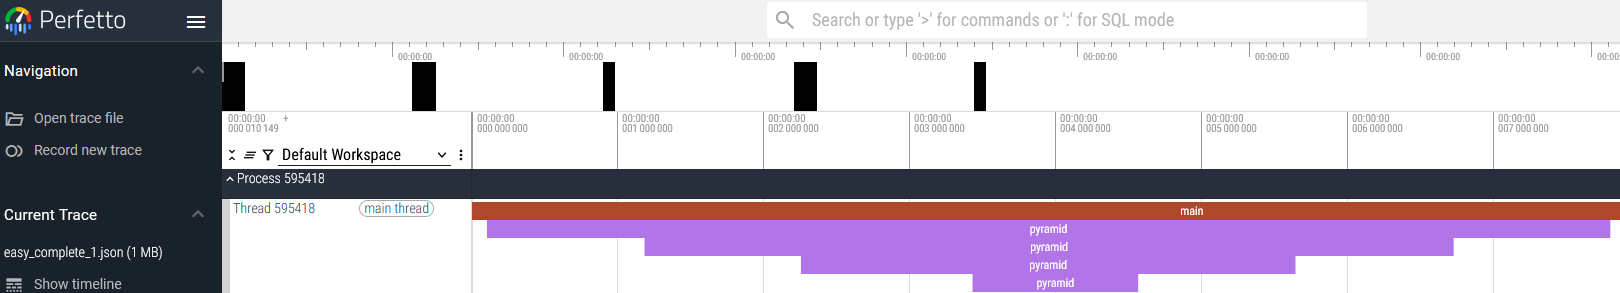
\includegraphics[width=\textwidth,height=0.7\textheight,keepaspectratio]{pics/cxxet/pyramid.png}
        \caption{Visualizing the `pyramid' example in perfetto.ui}
    \end{figure}

\end{frame}



\begin{frame}{cxxet features}{Resulting data format}
    Honoring \hyperlink{data_format}{requirement for data format}, small (mandatory) subset of google's `Trace Event Format'\footnote{https://docs.google.com/document/d/1CvAClvFfyA5R-PhYUmn5OOQtYMH4h6I0nSsKchNAySU/edit?tab=t.0} -> `JSON Object Format'\footnote{https://docs.google.com/document/d/1CvAClvFfyA5R-PhYUmn5OOQtYMH4h6I0nSsKchNAySU/edit?tab=t.0\#heading=h.q8di1j2nawlp} was chosen.

    Advantages:

    \begin{itemize}
        \item portability,
        \item `json':
        \begin{itemize}
            \item human readable (and most probably understandable too),
            \item easily processable by tools such as `jq', or custom written scripts.
        \end{itemize}
    \end{itemize}

    Disadvantages (compared to binary formats):

    \begin{itemize}
        \item not as compact,
        \item not as fast to write out.
    \end{itemize}

\end{frame}

\begin{frame}[fragile]{cxxet features}{Resulting data format example}
    \begin{lstlisting}[language=json]
{
    "displayTimeUnit": "ns",
    "traceEvents": [
        {"name": "main", "ph": "X", "ts": 10.199, "dur": 9935.55, "pid": 220013, "tid": 220013},
        ...
    ]
}
    \end{lstlisting}

\end{frame}

\begin{frame}{cxxet features}{Trace event format adoption}
    Currently, only fraction of the potential format features are implemented/used\footnote{https://docs.google.com/document/d/1CvAClvFfyA5R-PhYUmn5OOQtYMH4h6I0nSsKchNAySU/edit?tab=t.0\#heading=h.puwqg050lyuy}:

    \begin{itemize}
        \item `CXXET\_mark\_duration(...)' generates pair of `duration events',
        \begin{itemize}
            \item `CXXET\_mark\_duration\_begin(...)' generates only start duration event,
            \item `CXXET\_mark\_duration\_end(...)' generates only end duration event,
        \end{itemize}
        \item `CXXET\_mark\_complete(...)' generates `complete event',
        \item `CXXET\_mark\_instant(...)' generates `instant event' and fianlly
        \item `CXXET\_mark\_counter(...)' generates `counter event'.
    \end{itemize}

\end{frame}

\begin{frame}{cxxet features}{Resulting data visualization}
    For the resulting data visualization, "external" tool must be used, of which there are many, for example:

    \begin{itemize}
        \item chrome://tracing - built inside `google chrome' browser,
        \item https://ui.perfetto.dev/ - free web service
        \item Tracy - partial support, must be converted to its native format first,
        \item ...
    \end{itemize}

\end{frame}

\begin{frame}{cxxet features}{Collected data transfer}
    \hyperlink{writing_out_data}{Collected markers} are transfered accross those different boundaries:

    \begin{enumerate}
        \item within the application:
        \begin{enumerate}
            \item each marker put directly to `thread\_local' storage buffer,
            \item those buffers are handed over to the "global" one,
        \end{enumerate}
        \item writng the data out (e.g. to a file).
    \end{enumerate}

    All those actions and thread safe - point 1.1 is such by design, and points 1.2, 2 are protected by locking same instance of `std::mutex'.

\end{frame}

\begin{frame}[fragile]{cxxet features}{Writing the data to file programatically}
    Target filename can be specified programatically:

    \begin{lstlisting}[language=C++]
#include <cxxet/all.hxx>

int main(int argc, char const **argv) {
    char const *const filename{argc > 1 ? argv[1] : nullptr};
    CXXET_sink_global_flush(cxxet::output::format::chrome_trace, filename, true); // `true' means to defer the flush - in the destructor of the "global" buffer
    // ...
}
    \end{lstlisting}

\end{frame}

\begin{frame}[fragile]{cxxet features}{Writing the data to file using env. variable}
    Or environment variable `CXXET\_TARGET\_FILENAME' can be set to the desired filename, but `CXXET\_sink\_global\_flush(...)' must then be avoided:

    \begin{lstlisting}[language=bash]
$ CXXET_TARGET_FILENAME=/tmp/my_trace.json ./my_app_using_cxxet
...
    \end{lstlisting}

    \begin{lstlisting}[language=C++]
#include <cxxet/all.hxx>

int main(int argc, char const **argv) {
    // ... same as above ...
}
    \end{lstlisting}

    This has equivalent behavior as the previous example.
\end{frame}

\begin{frame}{cxxet features}{No external wrapper}
    It should be obvious from the previous slide(s) that no external wrapper/application is needed to obtain the profiling data. The `cxxet' library provides an self-contained solution to the collection of profiling data, such as `TracyClient' does, and saves it in a similar way to a file on a disk as `nsys' does.

\end{frame}

\begin{frame}{cxxet features}{Interoperability with threading, `fork' and similar}
    Finally, last requirement - being (easily?) manageable \hyperlink{fork_handling}{in `fork()'ing applications} - is fulfilled by functionality contained in `cxxet/sink\_diversion.hxx'\footnote{https://github.com/Ruzovej/cxxet/blob/main/include/public/cxxet/sink\_diversion.hxx}. Unfortunately, this functionality must be manually guarded by the `\#ifdef CXXET\_ENABLE', as in the simplified snippet from one example\footnote{https://github.com/Ruzovej/cxxet/tree/main/examples/usage/sink\_diversion} on next slide:

\end{frame}

\begin{frame}[fragile]{cxxet features}{Interoperability with threading, `fork' and similar - example snippet}
    \begin{lstlisting}[language=C++]
#ifdef CXXET_ENABLE
#include "cxxet/sink_diversion.hxx"
#endif
int main(int argc, char const **argv) {
#ifdef CXXET_ENABLE
  auto file_sink_local{cxxet::file_sink_handle::make(false)}; // `false' - not thread safe
  file_sink_local->flush(cxxet::output::format::chrome_trace, filename_custom, true);
#endif
  std::thread t1{[&]() {
#ifdef CXXET_ENABLE
    file_sink_local->divert_thread_sink_to_this();
#endif
    // ... `CXXET_sink_thread_reserve();' and regular code ...
  };
    \end{lstlisting}

\end{frame}

\begin{frame}{cxxet features}{Interoperability with threading, `fork' and similar - further explanation}
    In the example above, if the main thread initialized `cxxet' structures as usual (without diverting its "sink"), the application would have generated at least those 2 different trace files, independent of each other.

    This is true even if both "branches" called same function (e.g. `pyramid' :-) ) that contains any markers - they would be collected in the proper `thread\_local' buffer, which would get flushed to its parent sink:

    \begin{itemize}
        \item main thread -> default, "global" sink,
        \item thread `t1' -> `file\_sink\_local' sink.
    \end{itemize}

\end{frame}

\begin{frame}[fragile]{cxxet features}{Interoperability with threading, `fork' and similar - example snippet}
    Even though the example demonstrates data diversion only from different threads to their corresponding files, similar principles apply to processes after successful `fork()', with exception that currently unflushed data in child process's "global" sink should be discarded, for example as such:

    \begin{lstlisting}[language=C++]
// ...
if (fork() == 0) { // child process
  CXXET_sink_global_flush(cxxet::output::format::chrome_trace, nullptr, false); // `false' - don't defer the flush
  // same applies to "locally owned" sinks ...
  // take care - previous target file was overwritten in this process!
}
// ...
    \end{lstlisting}

\end{frame}

\begin{frame}[fragile]{cxxet features}{Interoperability with threading, `fork' and similar - example snippet}
    Any such "redirection" can be later reverted if needed:

    \begin{lstlisting}[language=C++]
// ...
file_sink_local->divert_thread_sink_to_this();
// ...
CXXET_sink_thread_flush(); // explicit flush is required + beware of unterminated markers in current scope!

CXXET_sink_thread_reserve(); // call this for less skewed measurement explicitly
CXXET_sink_thread_divert_to_sink_global(); // redirect `thread_local' buffer back to the global one
// ... more code with markers
    \end{lstlisting}

\end{frame}



\section{End of the talk}

\begin{frame}{Questions and discussion}
    \begin{center}
        \Large Thank you for your attention! And organizers of those meetups for giving me this opportunity.

        \vspace{1cm}

        Questions?

        \vspace{1cm}

        \texttt{ruzovej@gmail.com}

    \end{center}

\end{frame}

\end{document}
